
\chapter{Timeline of research activity}
\label{appendix:timeline}
\section{Engagement with Small Steps}
My research and engagement activity with Small Steps took place from February 2018 to September 2019 when they ceased activity. I began working from their offices for half of the week every week from March 2018 to August 2018. During this time I undertook three design research workshops with them, generally around the development of a peer support tool for young people with experience of homelessness. The first, "The Survival Agency", was a crude attempt at using gameful methods to explore tensions around the futures of youth support services. This was unsuccessful as an engagement tool. The two workshops focused on exploring issues around getting and receiving support through the use of a participatory persona creation tool, a self-guided workbook, and a workshop envisioning potentially useful technologies. The majority of my engagement with Small Steps was ethnographic. 

\section{Engagement with Building Bridges}
My research and engagement activity with Building Bridges took place from May 2018. I still maintain a relationship with them to this day, but I stopped collecting data for my PhD from them in 2020, as a result of the COVID-19 pandemic. I was part of the initial workshop designing the outline for the Building Bridges project in early June 2018. I then joined the team as a design researcher from this point. I developed a close friendship with Karen and Mandy over the life of the project, and met with them at numerous places around the country to work on projects relating to Building Bridges. As this was a national, remote team, my ethnography took place in these spaces, online or on phone calls, and during residentials. A residential took place in November 2018, January 2019, March 2019, and October 2019 (rearranged from June 2019). In the second cohort of the programme, residentials took place in November 2019, January 2020, and then the COVID-19 pandemic hit. Whilst further residentials took place eventually, I did not collect data for my thesis from them. 

Whilst the majority of my work with Building Bridges was ethnographic, the nature of my involvement with the programme was ostensibly about the use of the Gabber \cite{rainey_gabber_2019} participatory research tool for programme evaluation. The evaluation of the programme was conducted through the use of Gabber. This was a project that initially featured in this thesis, but this (and the participatory film-making and participatory user experience design projects) ultimately only constituted an exploration of the limits of existing participatory methods. Due to the length constraint of the thesis, I did not write a chapter exploring these three projects as many of the same lessons are learned through the \textit{It's Our Future} project with a greater level of insight.

\section{Engagement with Seabird}
My research and engagement activity with Seabird took place from August 2018 to April 2020, when their focus had to change to more active service delivery during the COVID-19 pandemic. I conducted a number of focused ethnographies with Seabird. I lived in the county they were based in for all of November 2018, February 2019, and April 2019, alongside a series of other, shorter visits. November 2018 acted as a sensitisation trip, building relationships with workers and young people and getting to know the ecosystem they existed in. February 2019's trip focused on a participatory user experience design project, in which I used methods for co-design in technology settings as a way to explore workers and young peoples' relationships to technology and how this related to their ideas of the future (whilst also leading to the creation of a new website). April 2019's trip focused on a participatory film-making project in which care-experienced young people were taught the requisite audio, video, and storytelling skills to make a film about their experiences of life story work. I conducted this with Rebecca Nicholson and James Hodge, two members of my PhD cohort with experience in education, film-making, and audio recording. 

I had planned follow-up engagement on the basis of the projects I worked on with Seabird, but their focus on active service delivery as a result of the pandemic means that these did not come to pass. These would have focused on exploring the \textit{It's Our Future} methods more deeply in the context of the prior work I had done with them and Tina's participation role. My design work with Seabird initially featured in this thesis, but this (and the participatory evaluation project) ultimately only constituted an exploration of the limits of existing participatory methods. Due to the length constraint of the thesis, I did not write a chapter exploring these three projects as many of the same lessons are learned through the \textit{It's Our Future} project with a greater level of insight.

\section{\textit{It's Our Future}}
\textit{It's Our Future} began as a project in August 2019, the event took place in October 2019, and the manifesto was published in November 2019. There had been a plan to pursue follow up engagement in early 2020, but this fell through due to the actions of The Charity described in chapter \ref{ch:7}.

\section{Interviews about social care and COVID-19}
When it became clear that I might not be able to pursue my initial research plan as a result of the COVID-19 pandemic, I set about establishing contingencies. During April 2020, in the early days of the pandemic, I organised a small number of interviews with social care workers (who I knew via previous projects, such as Building Bridges) to understand what their experiences were during the early days of the pandemic. I completed seven interviews focused on any changes they were noticing in the delivery of services or working practices, how they were coping as a result of the changes, and what their perception of how young people were responding to the lockdown was. Whilst the interviews were incredibly insightful and a valuable record of that moment in time, the ability to conduct a design project at distance provided a clearer end to the work that I had been developing, and as such these interviews do not feature in the thesis.

\section{\textit{fractured signals}}
\textit{fractured signals} took place from January 2021 to May 2021. The early part of this activity was centered on the design process, settling on a frame for the project, and designing artefacts and interactions. The project itself ran in the last week of March and the first week of April.

\chapter{\textit{It's Our Future} full manifesto}
\label{appendix:iof-manifesto}
This is the full \textit{It's Our Future} manifesto, edited only for the privacy of The Charity.
\includepdf[pages=-]{Images/Appendices/manifesto.pdf}

\chapter{Script for \textit{fractured signals} calls}
\label{appendix:fs-script}
This is the full script used on calls with participants of \textit{fractured signals.}
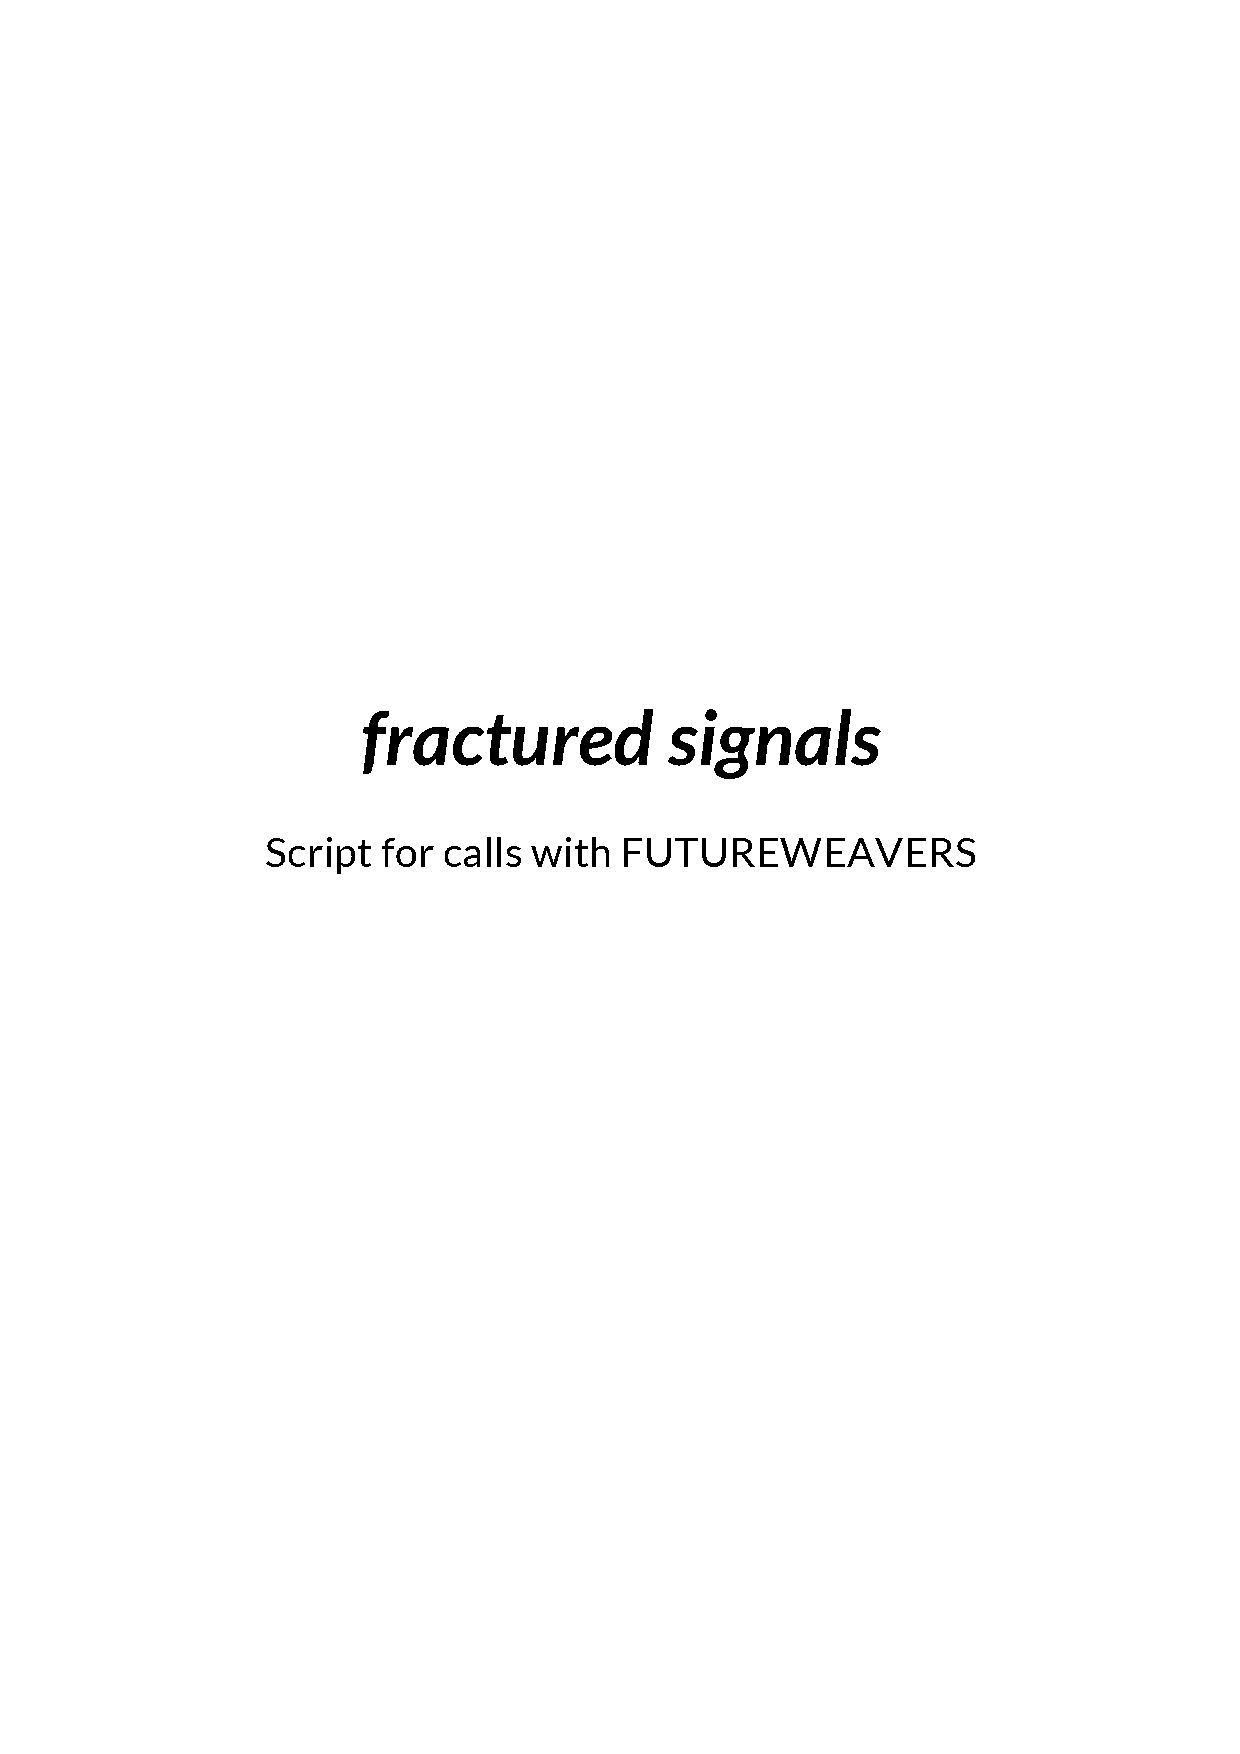
\includepdf[pages=-]{Images/Appendices/script.pdf}

\chapter{\textit{A Guide for New Futureweavers}}
\label{appendix:guide}
This is the full guide sent to participants of \textit{fractured signals.}
\includepdf[pages=-]{Images/Appendices/guide.pdf}

\chapter{Code for \textit{fractured signals} calls}
\label{appendix:code}
This is the full Node.js code used to determine the right call script to be used for \textit{fractured signals} participants.

\textit{\\Importing the express and Twilio libraries, and a .json file of the script}
\begin{verbatim}
const express = require('express');
const VoiceResponse = require('twilio').twiml.VoiceResponse;
const app = express();
const script = require('./script.json');
\end{verbatim}
\textit{Setting up a voice randomiser, so that each line of the script uses a different voice}
\begin{verbatim}
function say(twiml, text) {
    const voices = ['Polly.Brian-Neural', 'Polly.Emma-Neural', 
    'Polly.Amy-Neural', 'Polly.Joanna-Neural', 
    'Polly.Joey-Neural', 'Polly.Salli-Neural', 
    'Polly.Geraint', 'Polly.Raveena']
    let random = Math.floor(Math.random() * voices.length);
    twiml.say({ voice: voices[random]}, text);
}
\end{verbatim}
\textit{On the /fracturedsignals domain, work out the current day and determine whether to use the audio files for the fragmentation or the weaving}
\begin{verbatim}
app.get('/fracturedsignals', (req, res) => {
    //get date and send
    let now = new Date()
    let days = ["sunday", "monday", "tuesday", "wednesday", "thursday",
    "friday", "saturday"];
    if (now.getMonth() == 3){
        res.redirect('/fracturedsignals/fragment/' + days[now.getDay()] + "/0")
    } else if (now.getMonth() == 4){
        res.redirect('/fracturedsignals/weave/' + days[now.getDay()] + "/0")
    }
})
\end{verbatim}
\textit{For each line of the speech, say the line, and then select the next line to speak. If the line requires recording, record. If there is no next line, hang up.}
\begin{verbatim}   
app.get('/fracturedsignals/:week/:day/:speech', (req, res) => {
    let todayScript = script[req.params.week][req.params.day]
    const twiml = new VoiceResponse();
    let speech = req.params.speech;
    let nextSpeech = parseInt(req.params.speech) + 1
    if (speech <= (todayScript.length - 1)){
        console.log(todayScript[speech].text)
        say(twiml, todayScript[speech].text)

        if (todayScript[speech].record === true){
            twiml.record({action: '/fracturedsignals/' + req.params.week
                + '/' + req.params.day + '/' + nextSpeech, method: 'GET'})
            res.type('text/xml');
            res.send(twiml.toString());
        } else {
            twiml.redirect({method: 'GET'}, '/fracturedsignals/' + 
                req.params.week + '/' + req.params.day + '/' + nextSpeech)
            res.type('text/xml');
            res.send(twiml.toString());          
        }
    } else {
        twiml.hangup();
        res.type('text/xml');
        res.send(twiml.toString());      
    }
        
});
\end{verbatim}
\textit{Create a web server and listen for incoming requests.}
\begin{verbatim}
app.listen(3000);
\end{verbatim}
